\documentclass[a4paper]{article}
\usepackage{amsmath,amssymb,caption,float,graphicx,minted,xcolor}
\usepackage[utf8]{inputenc}
\usepackage[english]{babel}
% \usepackage[backend=bibtex]{biblatex}
% \addbibresource{Lab3.bib}
\captionsetup[figure]{labelsep=period}
\captionsetup[table]{labelsep=period}
\definecolor{bg}{rgb}{0.95,0.95,0.95}
% \renewcommand\thesection{\arabic{section}}
\usemintedstyle{emacs}
\begin{document}
\begin{center}
    \huge
    \textbf{ECE4810J\\System-on-Chip Design\\}
    \Large
    \vspace{15pt}
    \uppercase{\textbf{Homework 1}}\\
    \large
    \vspace{5pt}\today\\
    \vspace{5pt}
    Yihua Liu 518021910998
    \vspace{5pt}
    \rule[-5pt]{.97\linewidth}{0.05em}
\end{center}

Q1: Assume that we have 4 different processors on a SoC, each does 25\% of the application. If we improve two of the processors by 10 times, what would be the overall application speedup?

Assume the four parts of the application are done sequentially,
$$25\%*2*1/10+25\%*2=55\%$$
Thus, the overall application will speed up by 81.8\%. (If the four parts are parallel, the overall application will not speedup.)

Q2: Suppose that we have four different processors and all but one are totally limited by the bus. If we speed up the bus by 3 times and assume the processor performance also scales, what is the application speedup?

According to Amdahl's law,
\[Speedup\leq\frac{1}{\frac{T_{unaccel}}{T_{orig}}+\frac{T_{communication}}{T_{orig}}}.\]
Let $T_{orig}=1$, then
\[Speedup=\frac{1}{\frac{1}{4}+\frac{1}{3}\times\frac{3}{4}}=2.\]
Thus, the application speeds up 2 times.

Q3: A SoC uses 4-megabit memory chips and a 64-bit data bus. Draw a diagram and show the minimum number of memory chips we can use for each of the following chip configurations. What is the resulting minimum amount of memory (in bytes) we can use in a system for each chip configuration?\\
a. 4 Meg x 1\\
b. 1 Meg x 4\\
c. 256K x 16\\
a.
\begin{figure}[H]
    \centering
    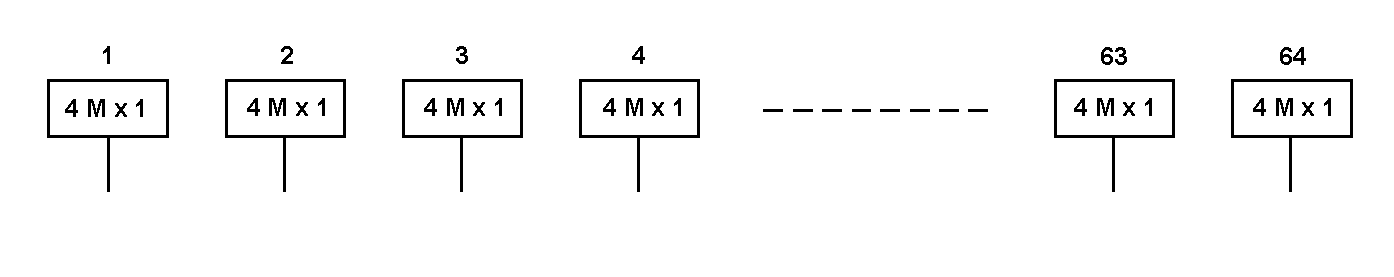
\includegraphics[width=1\textwidth]{3-a.pdf}
    \caption{Diagram of 4 Meg x 1 chip configuration.\protect\footnotemark[1]}
\end{figure}
Minimum number of memory chips = 64. Minimum amount of memory in bytes = 64 chips x 4 megabits/chip = 256 megabits = 32 megabytes.\\
\footnotetext[1]{If this figure and the following figures show improperly on your computer, please refer to the corresponding AI files attached.}
b.
\begin{figure}[H]
    \centering
    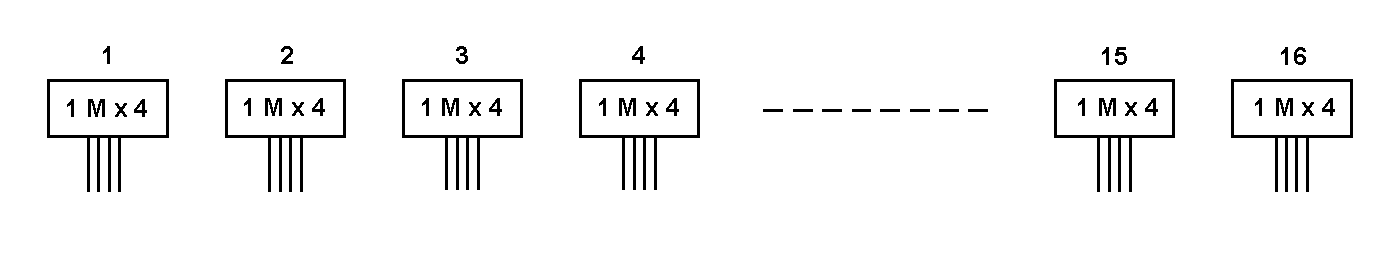
\includegraphics[width=1\textwidth]{3-b.pdf}
    \caption{Diagram of 1 Meg x 4 chip configuration.}
\end{figure}
Minimum number of memory chips = 16. Minimum amount of memory in bytes = 16 chips x 4 megabits/chip = 64 megabits = 8 megabytes.\\
c.
\begin{figure}[H]
    \centering
    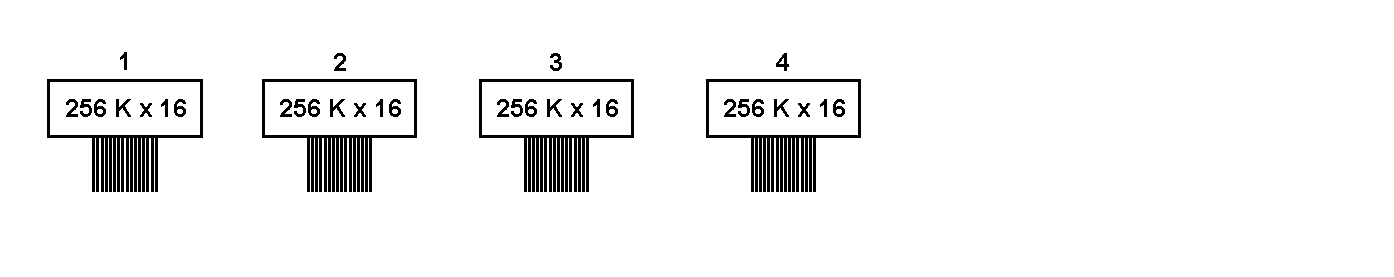
\includegraphics[width=1\textwidth]{3-c.pdf}
    \caption{Diagram of 256K x 16 chip configuration.}
\end{figure}
Minimum number of memory chips = 4. Minimum amount of memory in bytes = 4 chips x 4 megabits/chip = 16 megabits = 2 megabytes.

Q4: Hardware Acceleration, please answer the following questions based on your understandings.\\
1) You are designing a SoC using an Intel Xeon processor (host). Does it make sense to add an accelerator to implement the function z = ax + by + c? Explain.

Yes, it does. The function can be divided into three parts: loading the input, calculating, and saving the result in z. Adding an accelerator can reduce execution time by reading data from the processor, computing, and sending results back to the processor. It will be slow if the function is executed by the processor only.\\
2) You are designing a SoC using a CPU core with no floating-point support. Does it make sense to add an accelerator to implement the floating-point function? Explain.

Yes, it does. Similar to the function in a), the floating-point function can be divided and executed by the accelerator. It will be slow if the function is executed by the processor only.\\
3) You are designing a SoC using a high-performance embedded processor with a floating point unit. Does it make sense to add an accelerator to implement the floating-point function? Explain.

No, it does not. Since the high-performance embedded processor has already embedded a floating point unit, it will be very fast if the function is executed by the processor only. To add an accelerator is unnecessary.

Q5: In one of the lectures, we discussed static priority based arbitration scheme. Non-Preemptive Scheduling is when a task runs until it stops (voluntarily), or finishes. Preemptive Scheduling is where a task can be forcibly suspended. Let’s assume that we have the following four processes. Higher priority \# means more important.

1) If we use Non-Preemptive Scheduling, please draw diagram and show how scheduling works. Also calculate the average waiting time (AWT).
\begin{figure}[H]
    \centering
    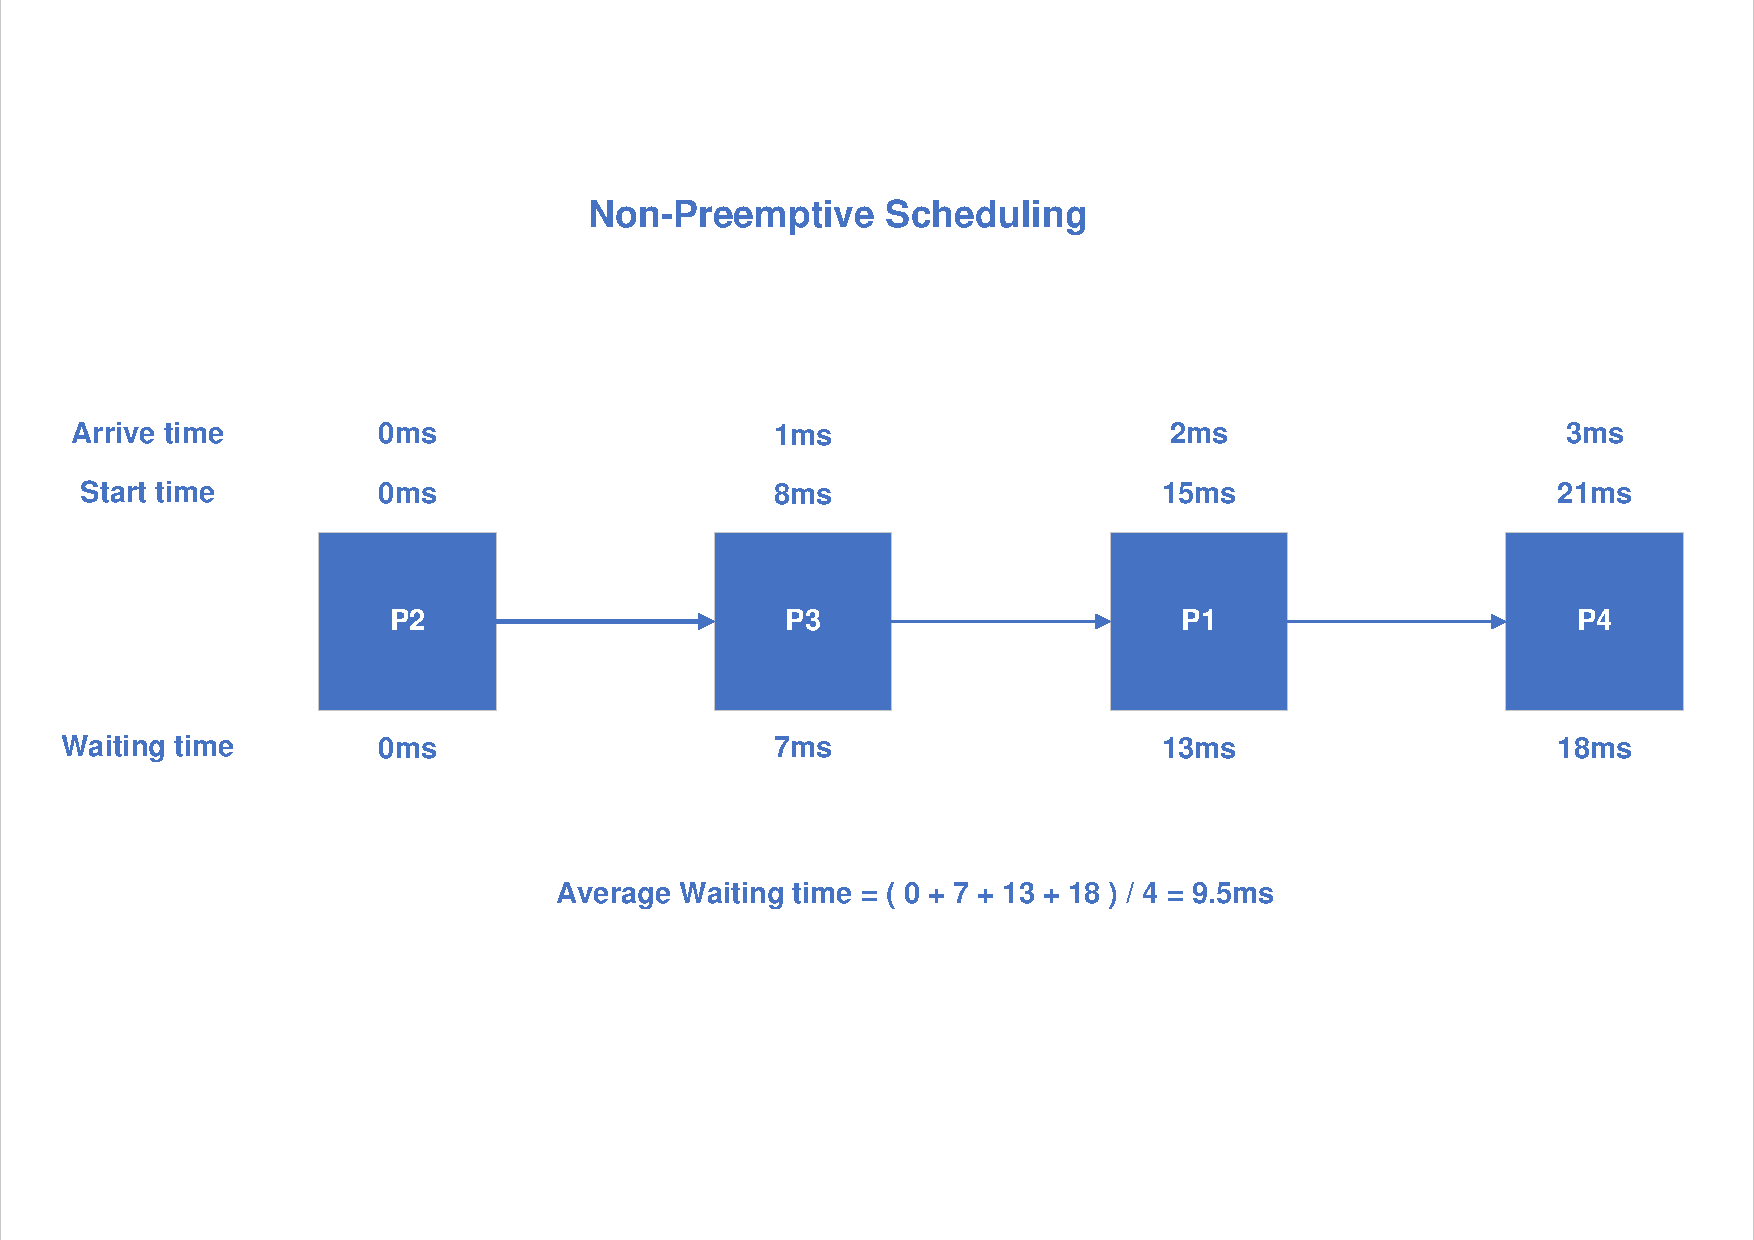
\includegraphics[width=1\textwidth]{5-1.pdf}
    \caption{Digram of Non-Preemptive Scheduling and its AWT.}
\end{figure}
2) If we use Preemptive Scheduling, please draw diagram and show how scheduling works. Also calculate the average waiting time (AWT).
\begin{figure}[H]
    \centering
    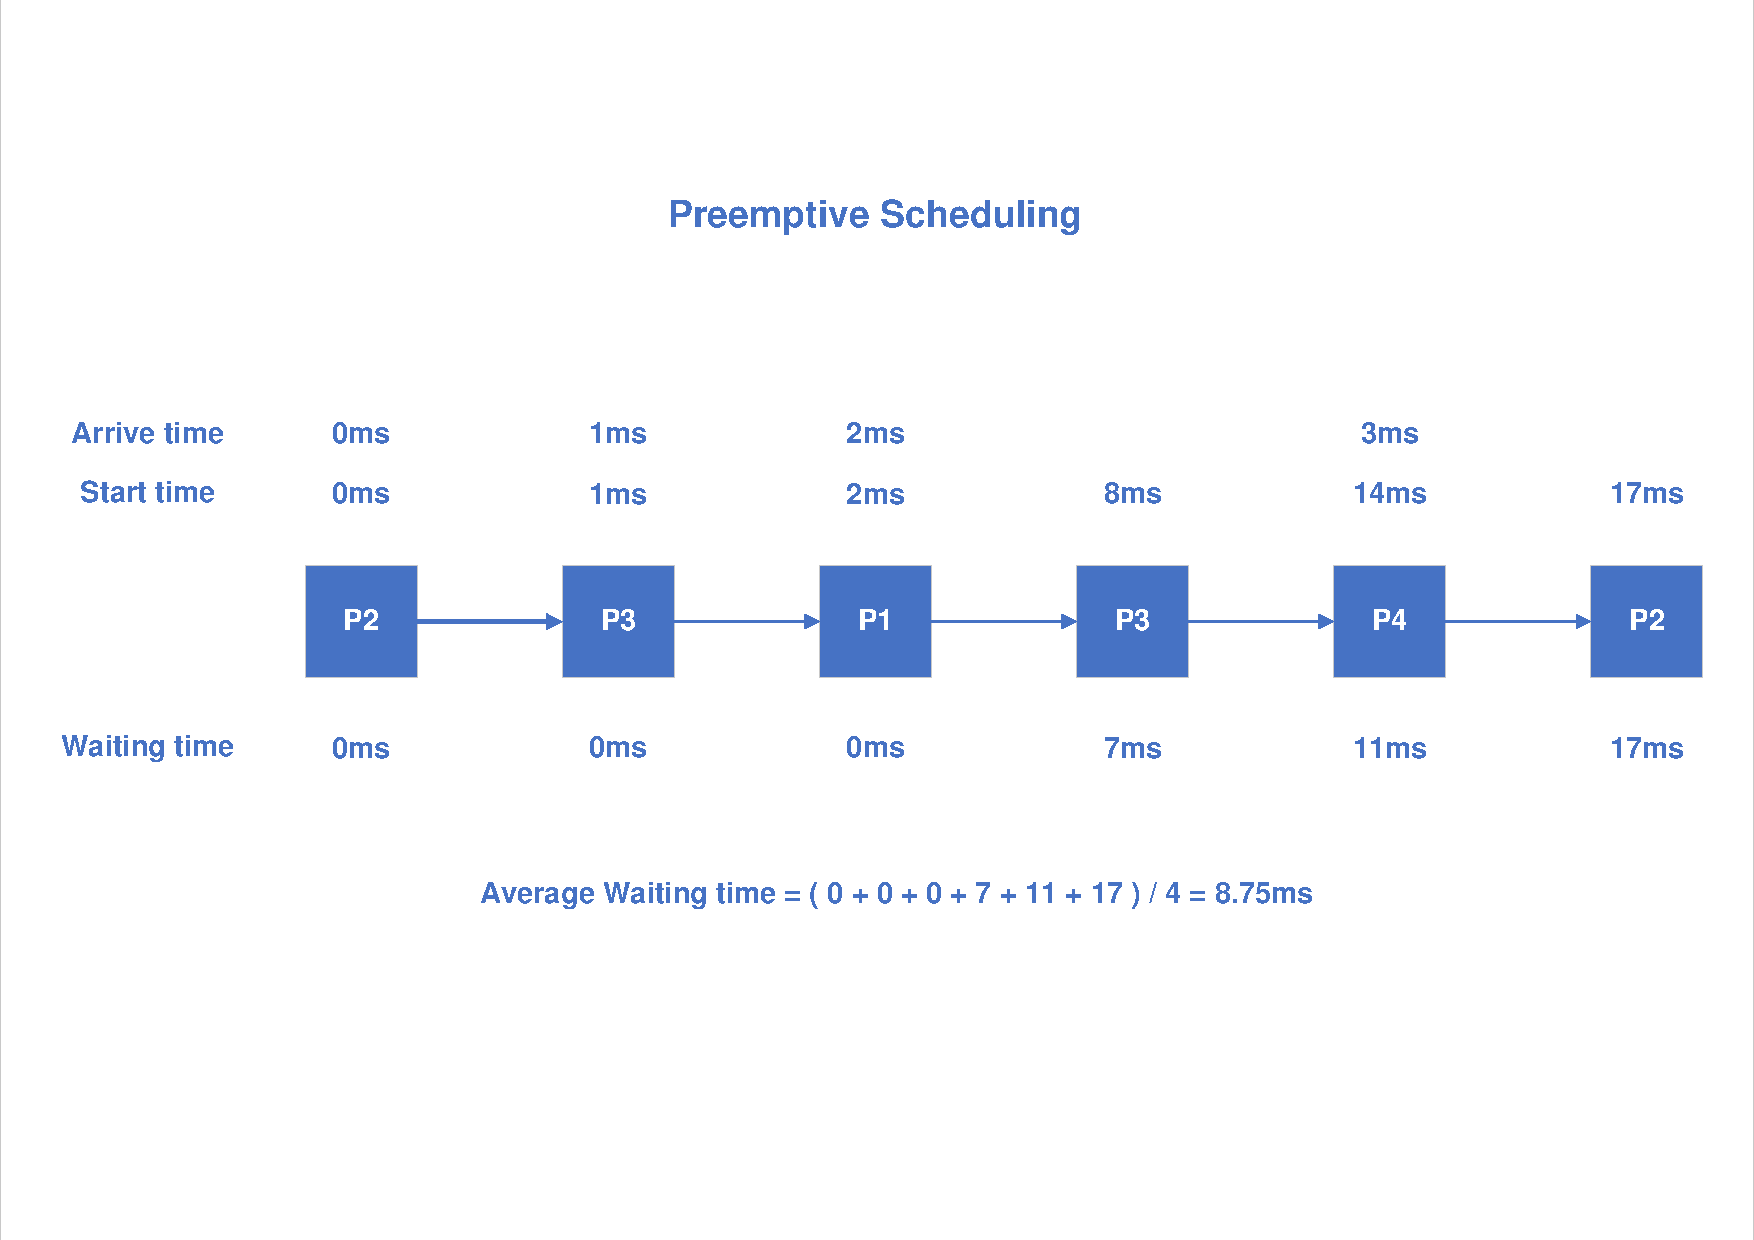
\includegraphics[width=1\textwidth]{5-2.pdf}
    \caption{Digram of Preemptive Scheduling and its AWT.}
\end{figure}

Q6: Consider two approaches of doubling the number of transistors on a SoC: halving the size of a single transistor while maintaining constant die area (Moore’s Law) versus maintaining the size of a single transistor while doubling the die area. List some reasons why the first approach is superior to the second approach.
\begin{itemize}
    \item The first approach uses less constant die area than the second approach, so the first approach costs less than the second approach.
    \item Larger size of a single transistor will cause more waste of die area.
    \item The first approach consumes less energy than the second approach. Chips made by the first approach have lower voltage and power than chipds made by the second approach.
\end{itemize}

Q7: For a chip product, the NRE cost and unit cost are the following for the four technologies.\\
1) Calculate total per-unit cost for production volume of 100, 1k, 10k and 100k units.
\begin{table}[H]
    \centering
    \begin{tabular}{|c|c|c|c|c|}
        \hline
        Technology&100 units&1k units&10k units&100k units\\
        \hline
        Semi-custom VLSI&\$2,005&\$205&\$25&\$7\\
        \hline
        ASIC&\$510&\$60&\$15&\$10.5\\
        \hline
        FPGA&\$170&\$35&\$21.5&\$20.15\\
        \hline
        Microcontroller&\$115&\$25&\$16&\$15.1\\
        \hline
    \end{tabular}
    \caption{Total per-unit cost for production volume of 100, 1k, 10k and 100k units.}
\end{table}

2) Plot these data in a single graph and determine the best choice of technologies for these production volumes to achieve the lowest per-unit cost.
\begin{figure}[H]
    \centering
    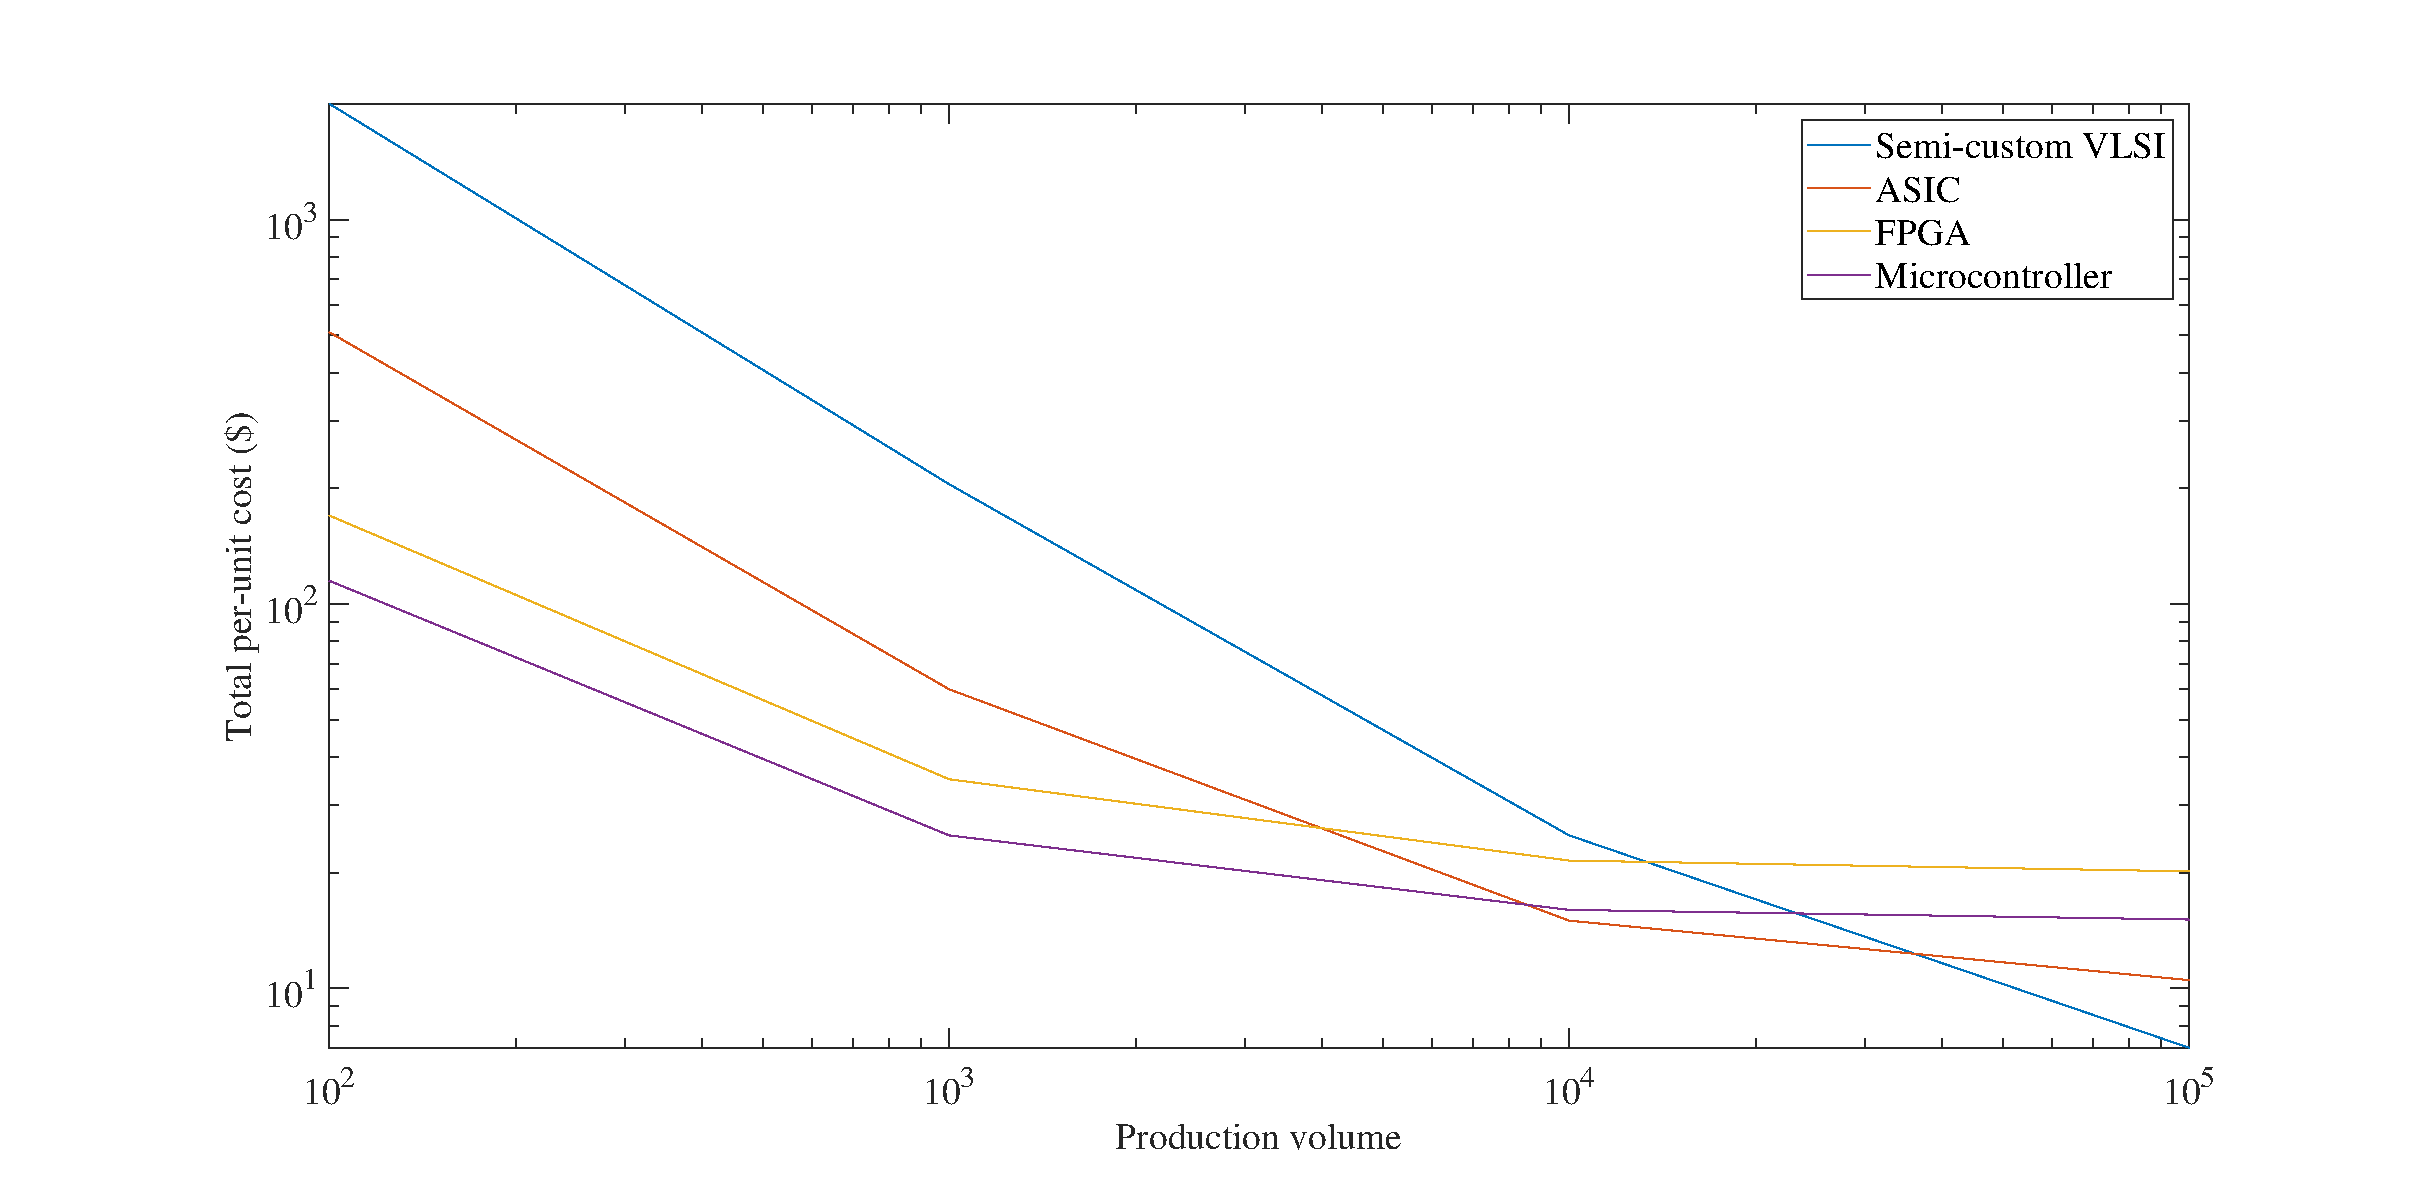
\includegraphics[width=1\textwidth]{7-2-1.eps}
    \caption{Semilogx plot of total per-unit cost for production volume of 100, 1k, 10k and 100k units.}
\end{figure}
\begin{figure}[H]
    \centering
    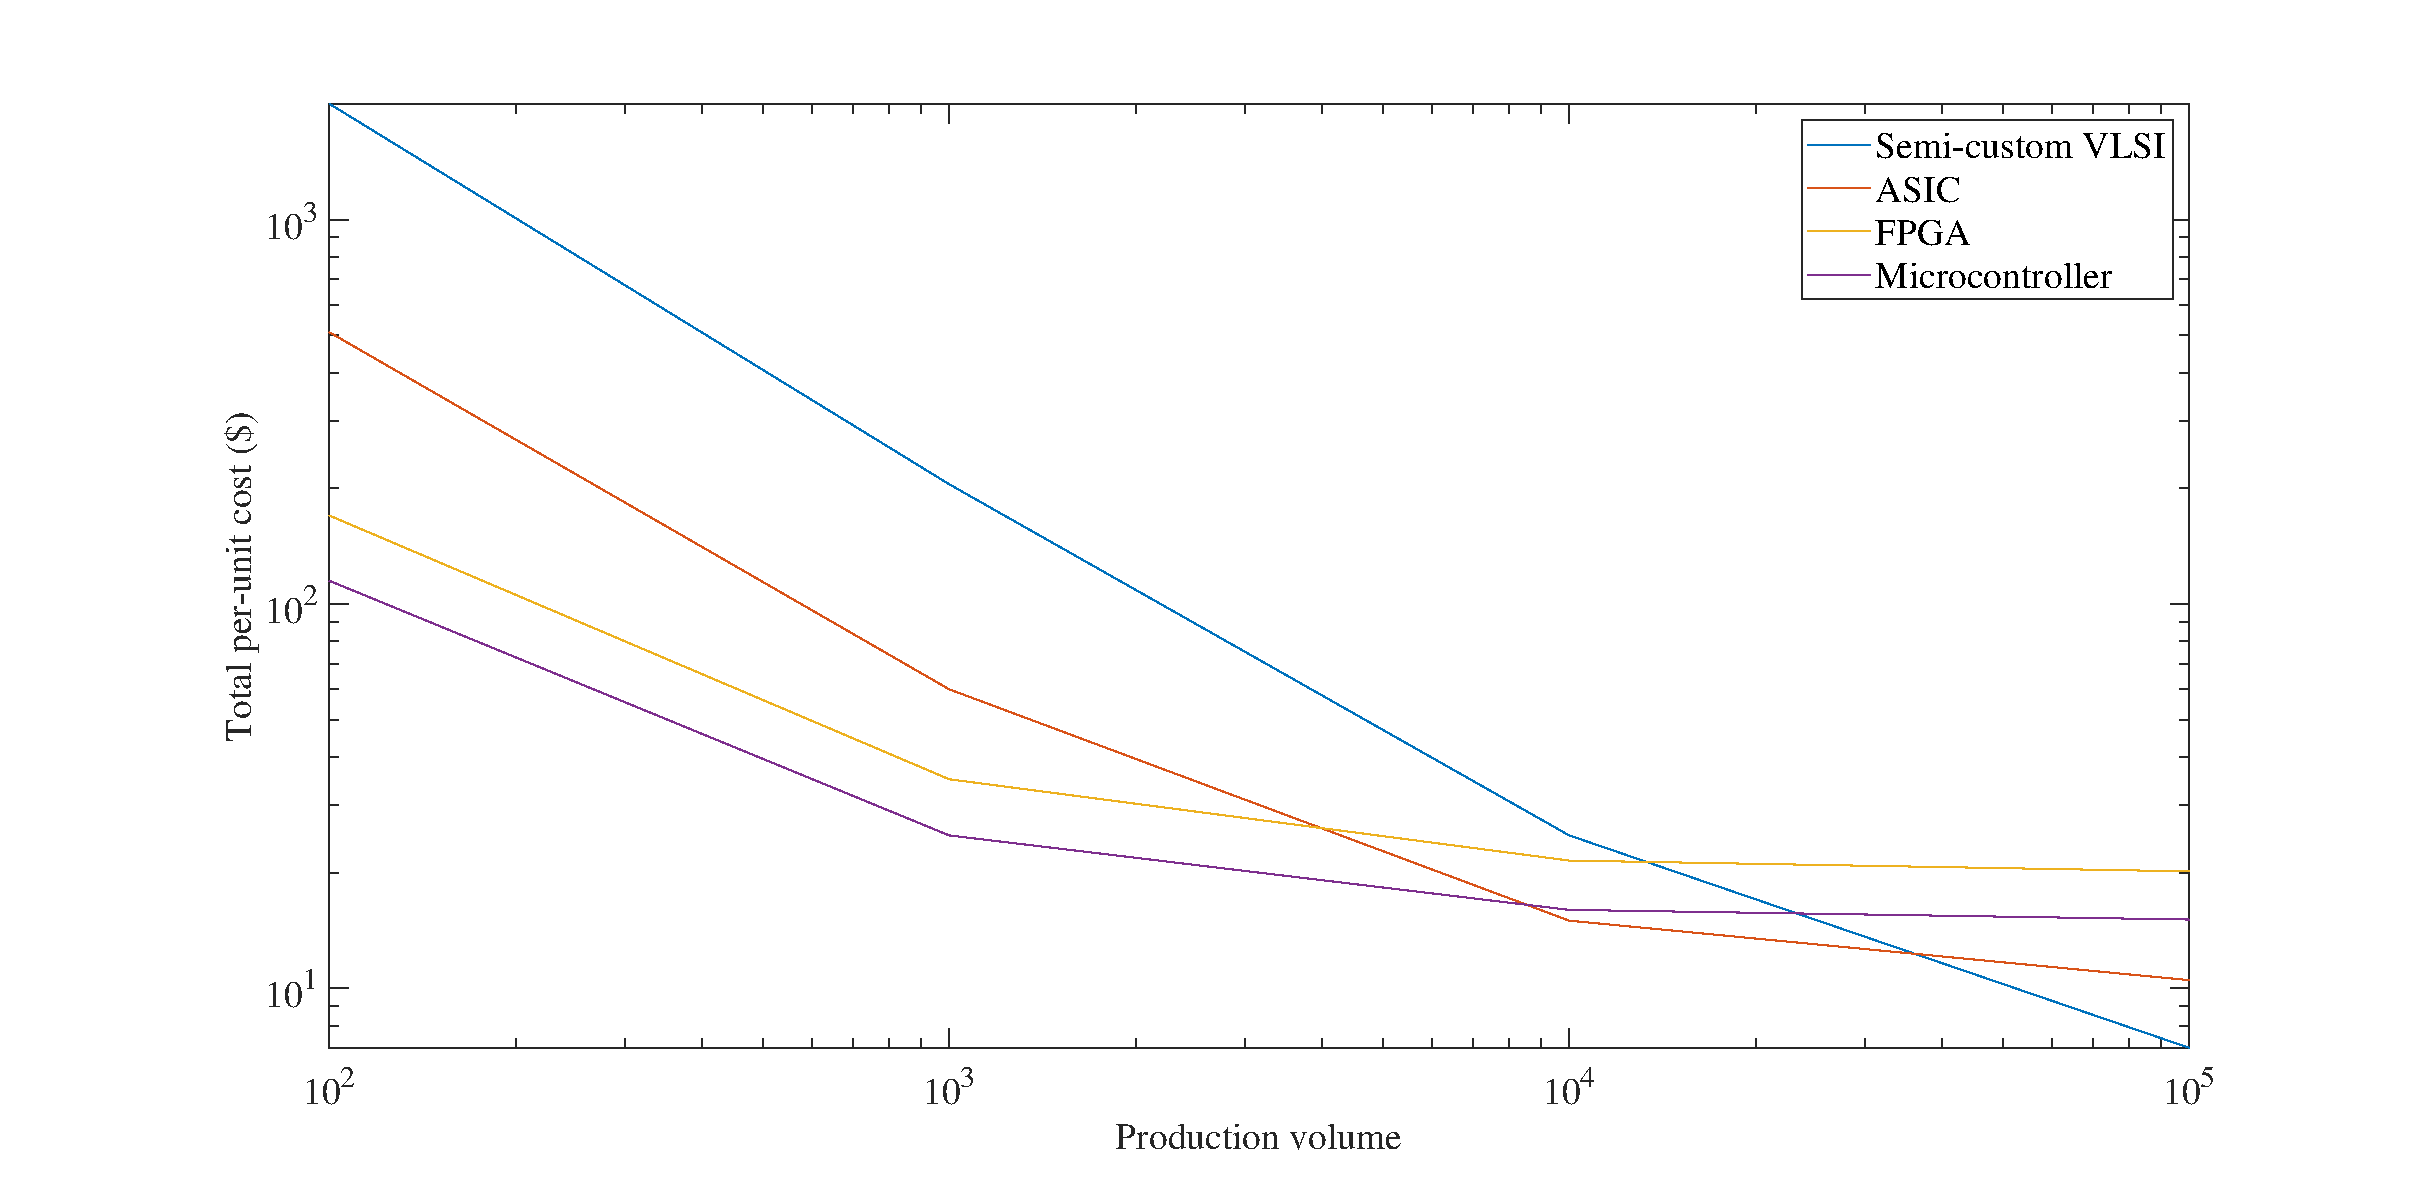
\includegraphics[width=1\textwidth]{7-2-2.eps}
    \caption{Loglog plot of total per-unit cost for production volume of 100, 1k, 10k and 100k units.}
\end{figure}
\noindent If the production volume $x=100$ or $x=1$k, choose microcontroller;\\
If the production volume $x=10$k, choose ASIC;\\
If the production volume $x=100$k, choose semi-custom VLSI.

3) Determine the range of production volumes for which each of these technologies is financially optimal.\\
Solving the equation
\[\frac{200000+5x}{x}=\frac{50000+10x}{x},\]
\[x=30000.\]
Solving the equation
\[\frac{10000+15x}{x}=\frac{50000+10x}{x},\]
\[x=8000.\]
If the production volume $0<x<8000$, choose microcontroller;\\
If the production volume $x=8000$, choose microcontroller or ASIC;\\
If the production volume $8000<x<30000$, choose ASIC;\\
If the production volume $x=30000$, choose ASIC or semi-custom VLSI;\\
If the production volume $x>30000$, choose semi-custom VLSI.
\inputminted[frame=single,bgcolor=bg,breaklines,linenos]{matlab}{hw1q7_2.m}
\end{document}